\documentclass[fleqn, a4paper]{article}
\usepackage[top=1.5in,bottom=1.5in,left=1.15in,right=1.15in]{geometry}
\usepackage{graphicx}
\usepackage{tikz}
\usetikzlibrary{automata, positioning, arrows}
\usepackage[export]{adjustbox}
\usepackage{float}
\usepackage{amsmath}
\usepackage{pgfplots}
\pgfplotsset{compat=1.15}
\usepackage[utf8]{inputenc}

\title{EE463 Static Power Conversion I 
-Simulation Project I}
\author{Nail Tosun, Yusuf Selim Karataş}
\date{November 2018}

\usepackage{natbib}
\usepackage{graphicx}

\begin{document}

\maketitle

\section*{Question 1}
In this question we investigated the effects of different discrete step sizes on simulation in Simulink environment. Firstly we built single phase diode rectifier which connected through Turkish electrical grid ($400 V_{l-l}$ ). We connect 3 470 $\mu$F capacitors to make output voltage smoother. 
\begin{figure}[H]
  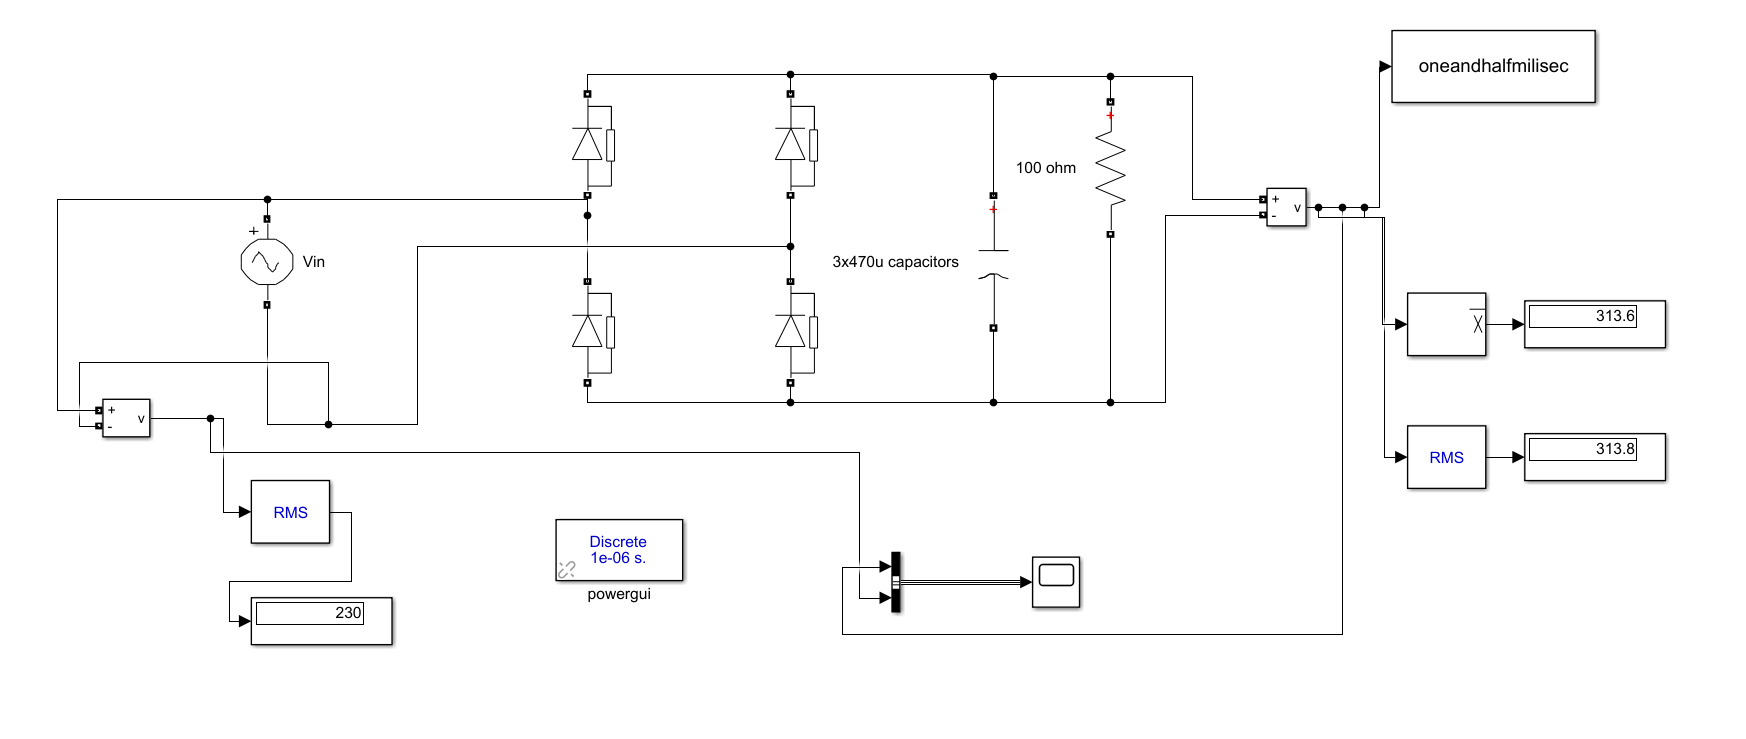
\includegraphics[width=\linewidth]{question-1-simulink-model.PNG}
  \caption{Simulink model of single phase diode rectifier}
  \label{fig:simulink2}
\end{figure}
\begin{figure}[H]
  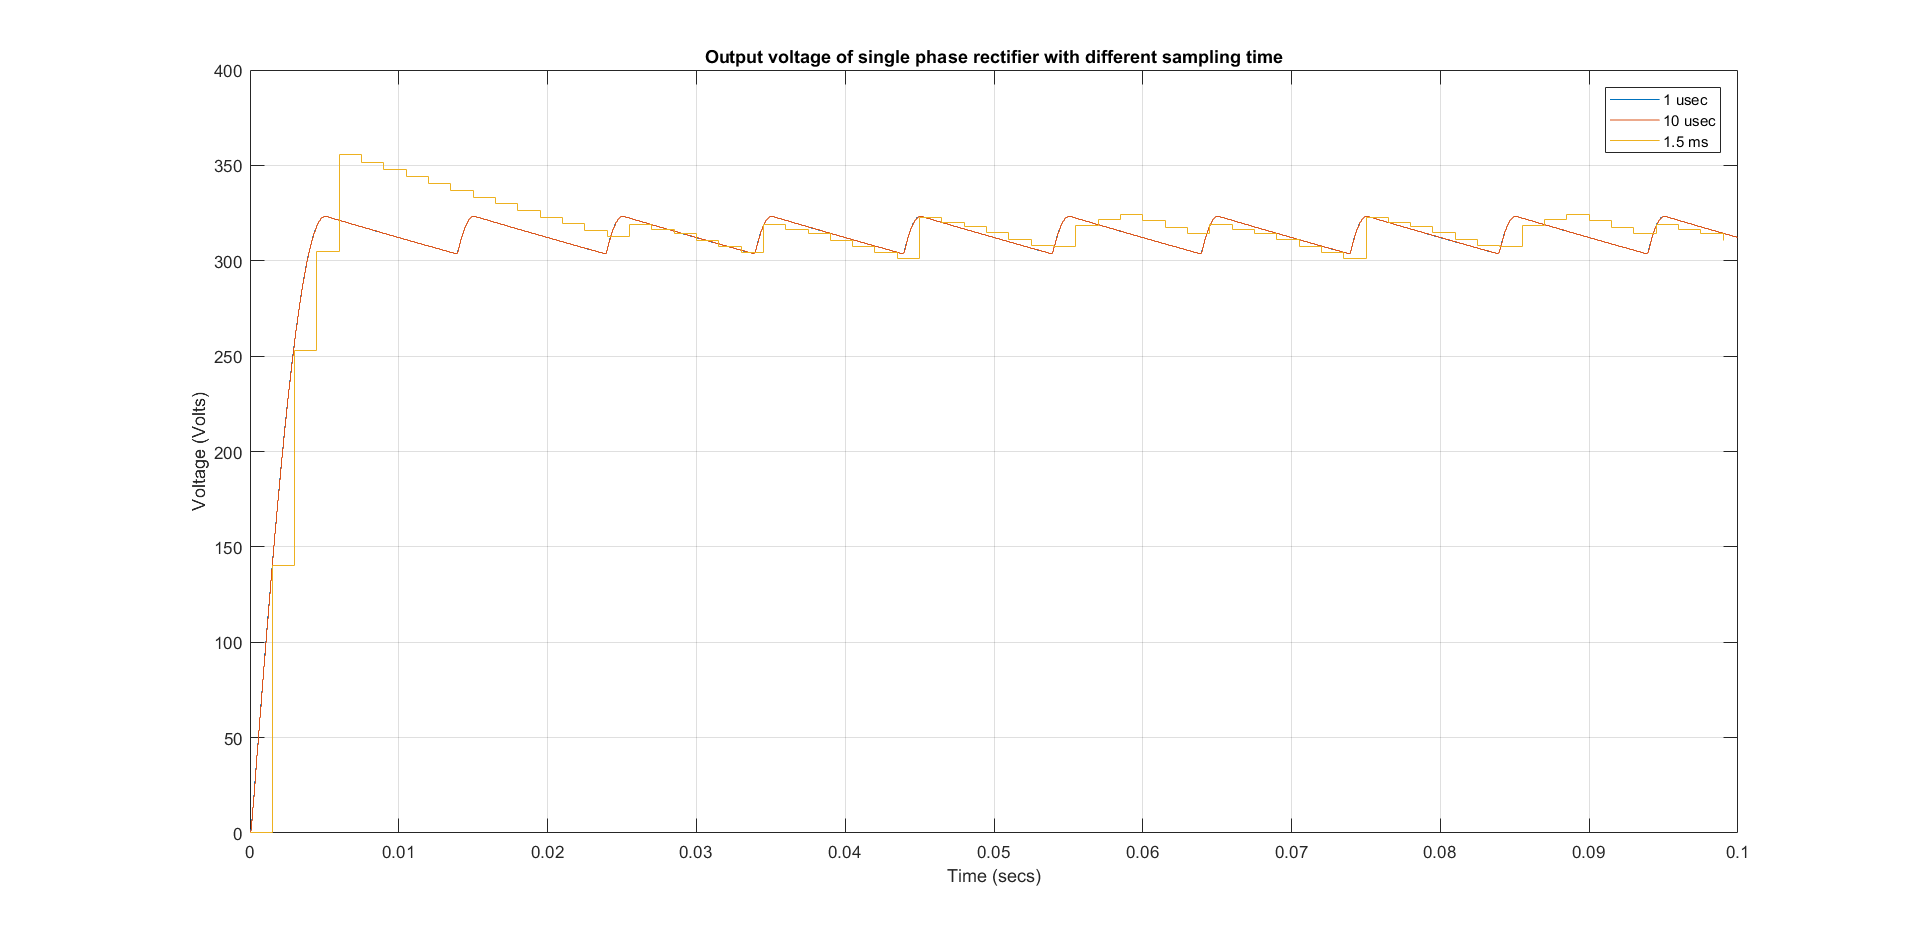
\includegraphics[width=\linewidth]{Q1_plots_different_samplings.png}
  \caption{Transients of voltage waveforms under various sampling frequencies}
  \label{fig:simulink2}
\end{figure}
\begin{figure}[H]
  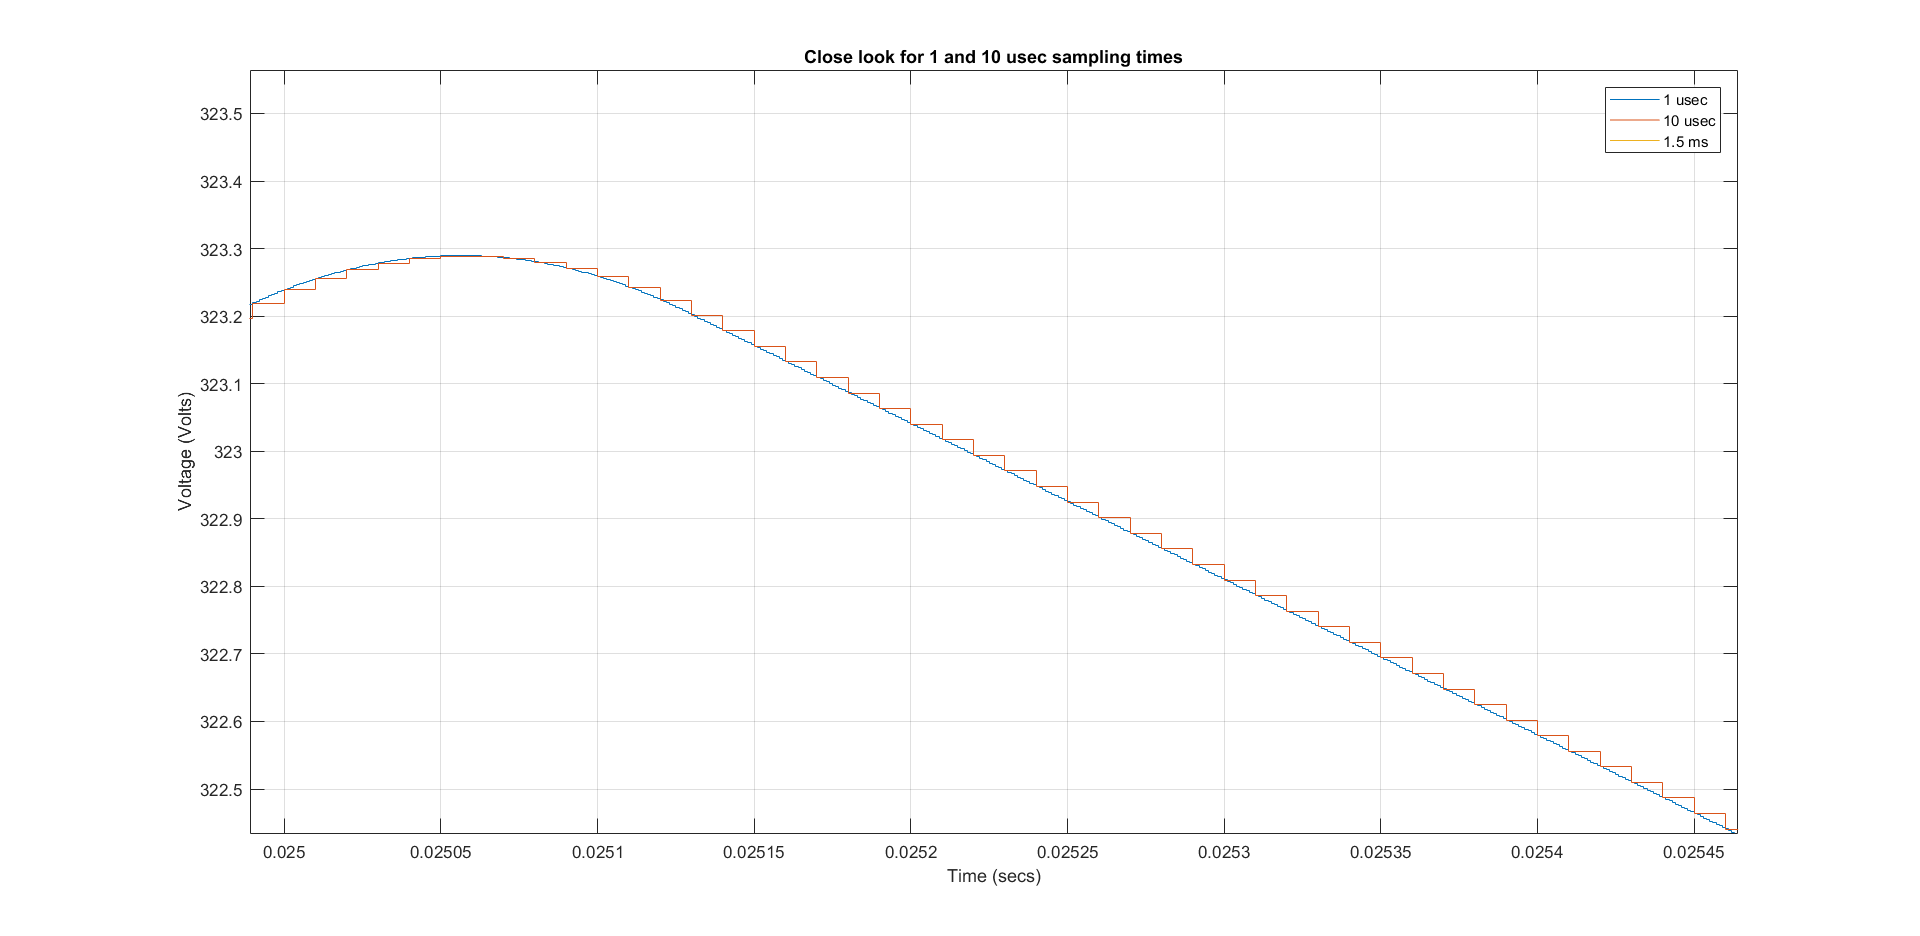
\includegraphics[width=\linewidth]{closer-look.png}
  \caption{Closer look for 1usec and 10usec to see transients}
  \label{fig:simulink2}
\end{figure}
We observed that, with large step size we lose some transients (especially at 1.5ms) but simulation time reduce since it is computationally inexpensive. With 50 Hz input signal there is no such difference between 1 $\mu$sec and 10 $\mu$sec however 1 $\mu$sec has 10 times more computational work. Therefore an engineer should do trade-off between resolution and computation time according his or her requirements.  
\section*{Question 2}
\subsection*{Part 2}
We choose MUR1540G with 15 A average current capability and 400 V peak repetitive reverse voltage. We make worst scenario for maximum current and peak reverse voltage. 
When line inductance 1H and R=25ohm. The maximum current 
\end{document}
